\section{Experiments}
\subsection{Case Studies}
We conduct four case studies to demonstrate descriptions generated by \ApproachName.
The IMDb movie dataset~\footnote{\url{https://www.imdb.com/}} has been used in plenty of works~\cite{DBLP:journals/tvcg/SrinivasanPEB18, DBLP:journals/pvldb/KrishnanWWFG16, DBLP:conf/ieeevast/BigelowNML19}.
We employ it to conduct our case studies.
We design and impltement a website to demonstrate our cases~\footnote{}.

\subsubsection{Case 1: Movies with Same Actors}\label{sec:imdb_movies}

% 我们挑选了数据集中2019年在中国上映的电影。
\textbf{1) Graph Wrangling}. We select movies in the dataset which is published in 2019 and is released in China.
% 我们保留了其中标题、发布日期、演员、类别、
We preserve seven attributes for movies: title, the publish date (\texttt{"date\_published"}), actors, genre, director, writer, and country.
Two movies are connected if they share at least one same actor.
We generate an attribute, \texttt{"shared\_actors"}, for each link. 
It records the number of shared actors.
We totally obtain 49 nodes and 99 links.
\textbf{2) Visual Encoding}. Nodes are visualized as \texttt{<circle>}s and links are visualized as \texttt{<line>}s.
The fill colors of \texttt{<circle>}s encode their publish seasons.
The width of \texttt{<line>}s encode the \texttt{"shared\_actors"}.
\textbf{3) Layout Computing}. We pre-compute a layout with a spring layout algorithm~\cite{DBLP:journals/spe/FruchtermanR91}.

The descriptions are generated for the created node-link diagram (Figure~\ref{fig:iMDBMovies}).
They can be separated into three parts:
\textbf{1) Linking Conditions.} Several conditions (e.g. ("C2", "country", "China"), ("C1", "year", "2019"), etc.) are detected but only the condition ("C2", "actors", "[arbitrary value]") is preserved because other conditions also are held on unconnected node pairs.
Thus \ApproachName~describes the linking condition as \textit{``Two nodes are connected if their attributes {\texttt{actors}} share an intersection''}.
\textbf{2) Visual Encodings.} All visual encodings are detected by \ApproachName~as expected.
Whereas, our technique does not detect that the color of each node encodes the published season because ``season'' is an abstract concept that are not under our consideration.
However, it generates the mapping of different color categories: \textit{``When the value of the attribute {\texttt{date\_published@month}} is {\texttt{04}}, {\texttt{06}}, or {\texttt{05}}, 
its {\texttt{fill}} turns to {\texttt{darkorange (\#ff7f0e)}}.$\ldots$''}, 
such that audience can obtain that the fill color encodes the ``season''.
\textbf{3) Layout Meanings.} \ApproachName~detects the nodes are placed with a topology-based layout, thus it describes the meaning of topology-based
layouts.

\begin{figure}
    \centering
    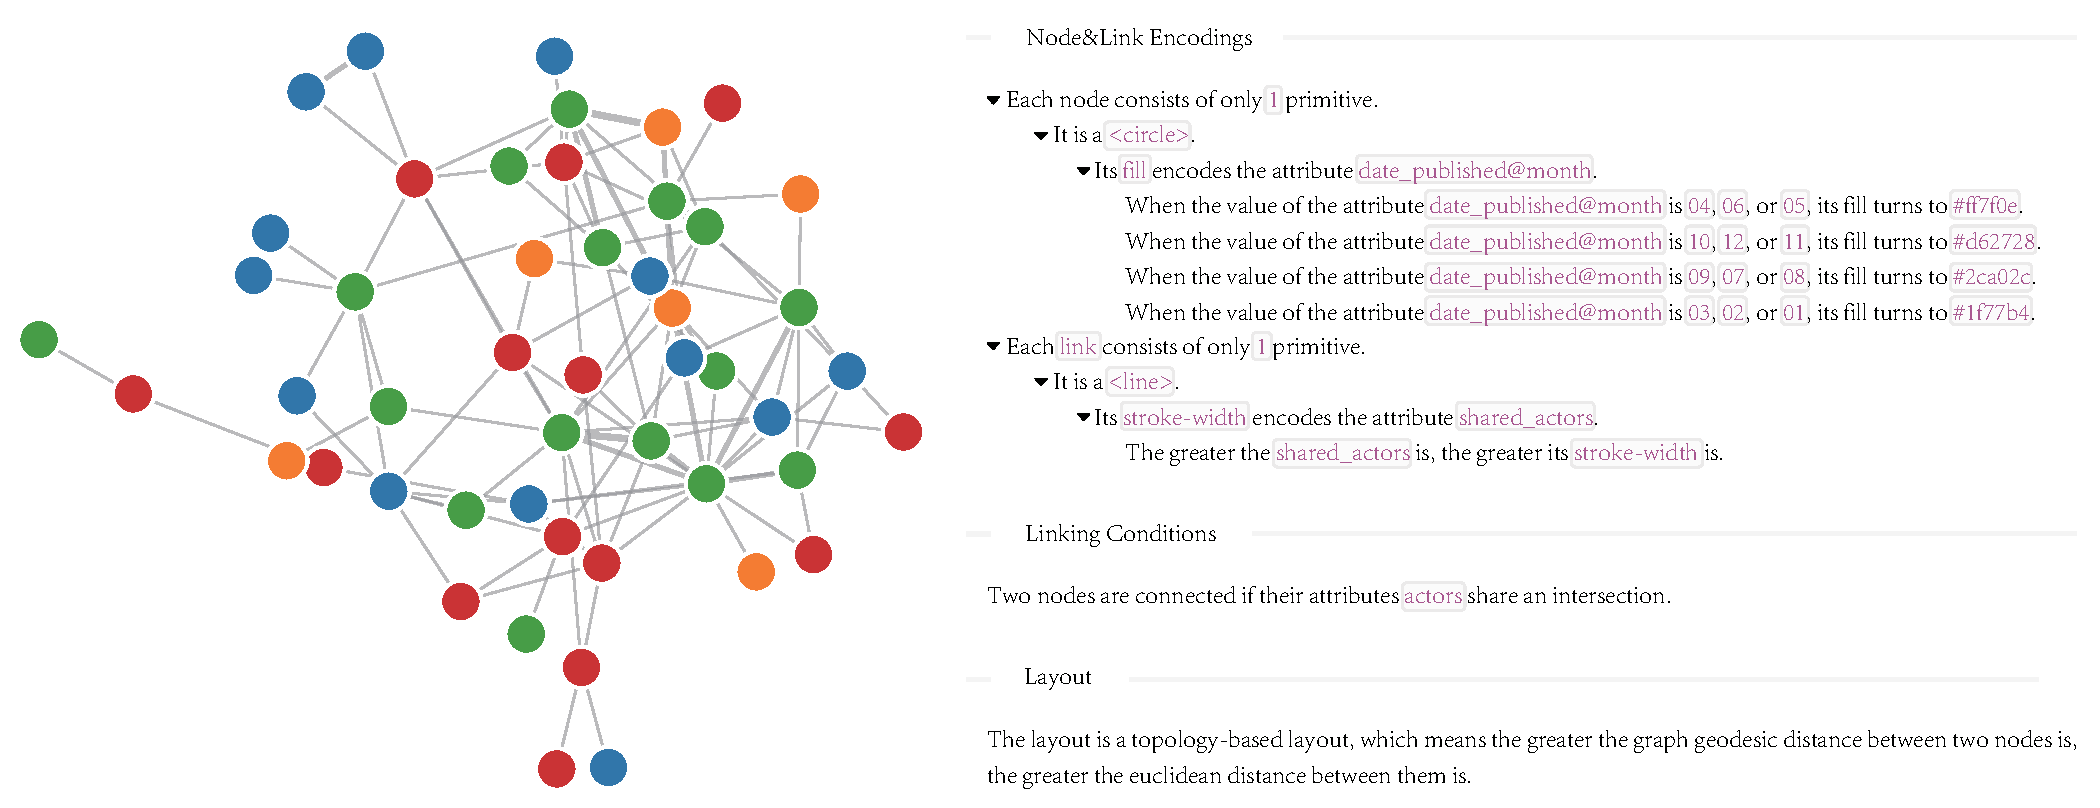
\includegraphics[width=1\columnwidth]{figures/iMDBMovies.eps}
    \caption{xxx}
    \label{fig:iMDBMovies}
\end{figure}


\subsubsection{Case 2: Actors with Same Movies}
With the IMDb movie dataset in Case~\ref{sec:imdb_movies}, we introduce another case which focuses on actors.

\textbf{1) Graph Wrangling}. We first select movies in the dataset that are only released in China from 2016 to 2021.
Their actors who have acted in more than five movies are regarded as nodes.
Each actor has five attributes: name, movies (s/he acted in from 2016 to 2021), the average vote (\texttt{"avg\_vote"}), the number of votes s/he got (\texttt{"votes"}), the number of movies in each year from 2016 to 2021 (\texttt{"number\_of\_movies\_by\_year"}).
Two actors are connected if they acted in at least one movie from 2016 to 2021.
We preserve the number of movies (\texttt{"number\_of\_shared\_movies"}) they both acted in in the link.
\textbf{2) Visual Encoding}. To show the activeness of each actor, we embed a simple line chart for each node to show the number of movies s/he acted in from 2016 to 2021. Similar to Case~\ref{sec:imdb_movies}, The width of \texttt{<line>}s encode its attribute \texttt{"number\_of\_shared\_movies"}.
\textbf{3) Layout Computing}. We utilize the layout to show two attributes (\texttt{"avg\_vote"} and \texttt{"votes"}) of each node. The x-coordinate encodes the attribute \texttt{"votes"} and the y-coordinate encodes the \texttt{"avg\_vote"}.

Different with Case~\ref{sec:imdb_movies}, in this case, each node consists of several primitives.
We distinguish primitives into different entities and classify primitives of one data entity into different roles.
We interpret the meaning of the line chart by describing its primitives (\texttt{<line>}s).

\subsubsection{Case 3: }

\subsubsection{Failure Cases}

\subsection{User Studies}
第一部分,找一些创作者,让他们阅读代码,为代码和节点链接图生成相应的描述;
通过让他们自己比较自己生成的描述和自动生成的描述,为描述进行打分。

第二部分,找一些不懂图可视化的人,让他们看生成的描述,回答一些问题。